\documentclass[11pt, oneside]{article}   	% use "amsart" instead of "article" for AMSLaTeX format
\usepackage{geometry}                		% See geometry.pdf to learn the layout options. There are lots.
\geometry{letterpaper}                   		% ... or a4paper or a5paper or ... 
%\geometry{landscape}                		% Activate for for rotated page geometry
\usepackage[parfill]{parskip}    			% Activate to begin paragraphs with an empty line rather than an indent
\usepackage{graphicx}				% Use pdf, png, jpg, or eps§ with pdflatex; use eps in DVI mode
								% TeX will automatically convert eps --> pdf in pdflatex	
\usepackage{amssymb}
\usepackage{amsmath}
\usepackage{listings}
\usepackage{color}

\date{}							% Activate to display a given date or no date

\newcommand{\tab} {\hspace*{2em}}
\newcommand{\stab} {\hspace*{.75em}}

\definecolor{codegreen}{rgb}{0,0.6,0}
\definecolor{codepurple}{rgb}{0.58,0,0.82}
\definecolor{codeblue}{rgb}{0,0,0.6}
\definecolor{codeorange}{rgb}{1,0.25,0}
\definecolor{backcolour}{rgb}{0.97,0.97,0.95}

\lstdefinestyle{gitlog}{
  backgroundcolor=\color{backcolour},
  breakatwhitespace=false, 
  breaklines=true,    
  keepspaces=true
  basicstyle=\ttfamily
  keyworkdstyle=\ttfamily
  commentstyle=\ttfamily
  identiferstyle=\ttfamily
  stringstyle=\ttfamily
  numbers=left,                    
  numbersep=5pt,  
}

\lstset{escapechar=/,style=gitlog}
\lstset{escapechar=_,style=gitlog}
\lstset{escapechar=\,style=gitlog}
\lstset{escapechar=',style=gitlog}
\lstset{escapechar=,,style=gitlog}

\begin{document}

\begin{center}
\LARGE
Stitch Language Final Reportd\\[2em]
\Large 
Daniel Cole (System Architect), Megan Skrypek (Tester), Rashedul Haydar (Manager), Tim Waterman (Language Guru)\\
\large dhc2131, ms4985, rh2712, tbw2105\\[2em]
\normalsize
December 22, 2015\\[3em]
\end{center}

\newpage

\LARGE\textbf{Introduction}\\[2em]
\normalsize
Most "modern" programming languages trace their origins back decades to before the advent of cheap, general purpose multicore CPUs.  They were designed for a distinctly mono-threaded environment.  While libraries and enhancements to mainstay languages such as C/C++ and Java have added multithreading capabilities, it remains in many ways bolted on kludge.  While newer frameworks such as Node.js provide more integral support for asynchronous operations, they lack the depth of support and power of a fully compiled language.  With Stitch, we aim to build a language that has the power and flexibility of a fully compiled C style language, while having native threading support for modern multithreaded applications.  Our goal is to create a translator from Stitch to C.\\[.5em]
Stitch is inspired by C, which has a very well known syntax, and has been one of the most widely used languages since it was released over forty years ago.  Stitch is a general purpose language that supports all standard mathematical and logical operations.  Like C, Stitch is strongly typed, and whitespace does not matter.  In addition to the standard C primitive types (\verb|int, double, char|, etc.)\\[.5em]
Stitch is able to provide an easy to use, clear paradigm for multithreaded operations by strictly limiting when and how they can be invoked.  This is done through the \verb|stitch| loop.  The body of this loop is automatically split into multiple threads, and the program will not continue until all threads have returned.  Using a simple loop paradigm, similar to well know control structures like \verb|while| and \verb|for| loops, allows for an easy learning curve, and clear easy to read code.  It also allows the complier to easily see what code needs to be run in a threaded manner, and to efficiently generate the threaded code.\\[.5em]
The underlying method by which Stitch runs multithreaded code is C's \verb|pthread| library.  The Stitch complier will wrap the body of the \verb|stitch| loop in a function.  This function will be executed in parallel using \verb|pthreads|.  Variable scoping inside the threads is also handled by the complier.  Each threads is passed a C \verb|struct| that contains all non-local variables needed by the block of code that is being multithreaded.  This prevents clobbering issues without needing to resort to \verb|mutex| locks.  The only exceptions to this rule are accumulators, which are very limited in scope, and arrays, which can be sliced and piecewise accessed by different threads concurrently.   

\newpage

\LARGE\textbf{Language Tutorial}\\[2em]
\normalsize

\newpage

\LARGE\textbf{Language Reference Manual}\\[2em]
\normalsize

\newpage

\LARGE\textbf{Project Plan}\\[2em]
\normalsize

\Large\textbf{Planning}\\[1em]
\normalsize
We arranged weekly meetings with our language advisor Professor Edwards to discuss progress and issues that we countered. The immediate feedbacks we received from him were extremely helpful in the development of the language, especially when we were heading in the wrong directions. We had weekly meetings as well where all of us got together and worked on the project. During the meetings we split up the work, often two people working together on the same thing. Initially this worked really well since all of us were new with OCaml. Later, we divided up the work on an individual level such as implementing some functionality or writing some specific tests.\\[3em]
\Large\textbf{Style Guide}\\[1em]
\normalsize
While programming our compiler we tried to follow these general guidelines:
\begin{itemize}
  \item Ocaml style guidelines, such as indentation and formatting
  \item Tried to keep lines limited to 80 characters, if this wasn?t possible due to unreadability, then we used 120 characters as the hard limit.
  \item Unlike Ocaml, we named variables in all lowercase and used underscores as a delimiter
  \item Used 4-space indentation for each program \ldots
\end{itemize}
\newpage
\Large\textbf{Project Timeline}\\[0em]
\normalsize
\tab\begin{description}
  \item[September 30] Proposal submitted
  \item[October 26] LRM submitted, scanner and parser with 1 shift/reduce error
  \item[November 16] Working scanner, parser, ast without arrays/stitch loops, \\[.5em]'Hello, Word' works
  \item[November 30] Finished semantic analyzer and cast
  \item[December 8] Finished c code generator with arrays added
  \item[December 14] Stitch loops working 
  \item[December 21] Final Presentation
  \item[December 22] Code cleanup and Final Report submitted \ldots
\end{description}
\tab\\[3em]
\Large\textbf{Team Roles and Responsibilities}\\[1em]
\normalsize
\tab\begin{tabular}{l c l}
Rashedul Haydar & - & Manager\\
Tim Waterman & - & Language Guru\\
Dan Cole & - & System Architect\\
Megan Skrypek & - & Tester\\
\end{tabular}\\

While we had assigned roles, the responsibilities became much more fluid as the project progressed. During the initial planning phase we all discussed the structure and components of the language. Later on, we also worked together on the semantic analyzer, C generator, and the variety of tests used for the test suite.
\newpage
\Large\textbf{Software Development Environment}\\[1em]
\normalsize
\begin{itemize}
  \item Version Control
  \begin{itemize}
    \item Git
  \end{itemize}
  \item Languages
  \begin{itemize}
    \item OCaml (4.02.3) for parser, scanner, ast, semantic analysis
    \item GCC for compiling generated C code
    \item bash for test suite and singer
    \item Python (2.7.5) for image curve generator
    \item \LaTeX\ for reports and documentation
  \end{itemize}
  \item Text Editors \ldots
    \begin{itemize}
    \item VIM
    \item Sublime
    \end{itemize}
\end{itemize}

\newpage
\Large\textbf{Project Log}\\[1em]
\normalsize
\lstinputlisting[style=gitlog]{commits.txt}

\newpage
\LARGE\textbf{Architectural Design}\\[2em]
\normalsize
\Large\textbf{Block Diagram}\\[1em]
\normalsize
\centerline{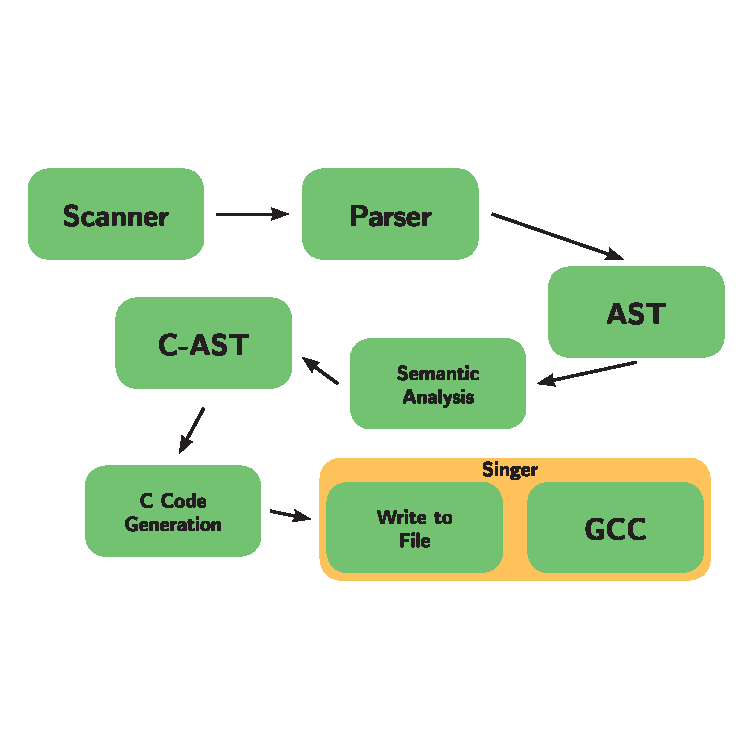
\includegraphics[scale=1.2]{block.pdf}}

\newpage
\Large\textbf{Interface Description}\\[1em]
\normalsize
\begin{tabular}{ l p{12cm} }
Scanner\\\verb|stch_scanner.mll| & The scanner is written in OCamlLex.  It takes input from the source file, and tokenizes it into keywords, identifiers, and literals.  It scans over and removes both single line and multi-line comments, as well as all whitespace not in string literals.  Any token that is not a keyword, or does not meet the criteria for an identifier or literal will throw a scanner error.\\[.5em]
Parser/AST\\ \verb|stch_parser.mly|\\\verb|stch_ast.ml| & The parser is written in OCamlYacc.  It takes the tokens from the scanner, and using the grammar defined in the parser and the datatypes defined in the AST, generates an abstract syntax tree.  The rules in the parser insure that code that passes this step is syntactically correct, although not necessarily semantically correct.  Any error at this stage will throw a syntax error.  The AST file also contains pretty printing functions for all datatypes defined therin.\\[.5em]
Semantic Checking/CAST\\ \verb|stch_ast.mll|\\\verb|stch_semantic.ml|\\\verb|stch.cast.mli| & Stitch first runs the AST through the semantic analyzer.  This pass insures that the code is semantically valid.  The output of the semantic analyzer is another AST, a C language AST.  The major difference here is that the CAST carries with it a Stitch Environment, which has, most importantly, a list of declared functions, and a symbol table, which contains all declared identifiers and their type.  Stitches symbol table also contains information on the expression that the identifier references, which is used in the C code generation to build pthread related code.\\[.5em]
\end{tabular}
\newpage
\begin{tabular}{ l p{12cm} }
Code Generation\\\verb|c_generator.ml| & The CAST, which as already been semantically analyzed is now pretty printed.  The bulk of the work to add multithreading is done here.  The C generator performs multiple passes on the CAST.  First any non-\verb|main| functions are printed.  Then any \verb|stitch| loops are analyzed, and their statements are turned into a function.  Finally, \verb|main| is printed.  This insures proper scoping of functions, and that all functions declared before main can be called in any Stitch block.  To convert \verb|stitch| loops to multithreaded \verb|pthread| code, the C generator first takes the body of the loop and transforms it into a function.  The generator also builds a custom \verb|struct| for each \verb|stitch| loop, that contains all in-scope, non-local variables that the loop will need access too.  It then generates the \verb|pthread| specific code, as well as a \verb|for| loop that creates and runs the threads.  The function containing the code body, as well as the structure containing all needed variables is passed into the \verb|pthread|.
\end{tabular}
\newpage


\LARGE\textbf{Test Plan}\\[2em]
\normalsize

\newpage

\LARGE\textbf{Lessons Lerned}\\[2em]
\normalsize

\newpage

\LARGE\textbf{Code}\\[2em]
\normalsize

\end{document}
